\documentclass{beamer}

%导言区
\usepackage[UTF8,noindent]{ctexcap}	
\setCJKsansfont[ItalicFont={华文新魏}]{黑体}

\usepackage{tikz}
\bibliographystyle{apalike}
\newtheorem{thm}{定理}
\renewcommand\proofname{证明}

\logo{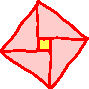
\includegraphics{logo.pdf}}

\usetheme{PaloAlto}


\title{勾股定理杂谈}
\subtitle{数学史讲座之一}
\institute{九章学堂}
\author{XuFr}
\date{\today}
\subject{勾股定理}
\keywords{勾股定理,历史}
%正文
\begin{document}
	\begin{frame}
		\titlepage%等价于\maketitle
	\end{frame}
	\begin{frame}{目录}
		\tableofcontents
	\end{frame}
	\section{勾股定理在古代}
	\begin{frame}{古希腊数学}
		勾股定理在西方称为毕达哥拉斯定理,古希腊数学家在 2000 多年前就已经发现并证明了它 \cite{Kline}。
		\begin{itemize}
			\item 公元前 6 世纪,毕达哥拉斯学派发现一个法则,可以构造直角三角形的边长。
			\item 公元前 3 世纪,欧几里得《几何原本》 使用面积法证明勾股定理。
		\end{itemize}
	\end{frame}
	\begin{frame}{古中国数学}{定理发现}
		中国早在 3000 多年前就知道勾股数的概念,比古希腊更早一些。
		
		《周髀算经》 的记载:
		\begin{itemize}
			\item 公元前 11 世纪,商高答周公问:
			\begin{quote}
				\zihao{-5}\kaishu
				勾广三,股修四,径隅五。
			\end{quote}
		\end{itemize}
	\end{frame}
\begin{frame}{古中国数学}{定理发现}
	中国早在 3000 多年前就知道勾股数的概念,比古希腊更早一些。
	
	《周髀算经》 的记载:
	\begin{itemize}
		\item 公元前 11 世纪,商高答周公问:
		\begin{quote}
			\zihao{-5}\kaishu
			勾广三,股修四,径隅五。
		\end{quote}
		\item 又记载公元前 7--6 世纪陈子答荣方问,表述了勾股定理的一般形式:
		\begin{quote}
			\zihao{-5}\kaishu 
			若求至日者,以日下为勾,日高为股,勾股各自乘,并而开放除之,得邪至日。
		\end{quote}
	\end{itemize}

\end{frame}
	\begin{frame}[t]{古中国数学}{定理发现}
	有论者认为早在公元前11世纪商高即已证明勾股定理\cite{quanjing}。完整地证明了见于三国时期 (公元前 3 世纪) 赵爽对 《周髀算经》 注释。
	\begin{figure}[ht]
		\centering
		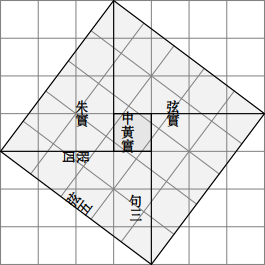
\includegraphics[scale=0.6]{xiantu.png}
		\caption{宋赵爽的弦图可给出勾股定理的一个富于对称美的证明}
		\label{fig:xiantu}
	\end{figure}
	\end{frame}
	\section{勾股定理在现代}
	\begin{frame}{现代叙述}
		\begin{thm}[勾股定理]
			直角三角形斜边的平方等于两直角边的平方和。可以用符号语言表述为:设直角三角形 ABC ,其中 $\angle{C}=90^{\circ}$,则有 \begin{equation}\label{eq:gougu}
				AB^2 = BC^2 + AC^2.
			\end{equation}
			\begin{center}
				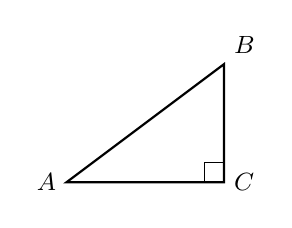
\begin{tikzpicture}[scale=0.5,font=\small]
				\draw[thick] (0,0) node[left] {$A$}
				-- (4,0) node[right] {$C$}
				-- (4,3) node[above right] {$B$} -- cycle;
				\draw (3.5,0) |- (4,0.5);
				\end{tikzpicture}
			\end{center}
		\end{thm}
	\end{frame}
	\begin{frame}{参考文献}
		\bibliography{math}
		\nocite{Shiye}
		\bibliographystyle{apalike}
	\end{frame}

\end{document}